\newpage
\section{Collaborative filtering}
Collaborative filtering is the process of filtering items based on others items with similar attributes.
\\\\needs more explanation\\\\
What is collaborative filtering.
\cite{RecommenderSystems:2}
\subsection{Content based}

\paragraph{}In content based recommender systems we try to make recommendations based on features we know. There are two types of content based recommender systems. 

\paragraph{}On the one hand we have the user based recommendation. This recommendation is done by trying to match users profiles, in order to find which item the user i might like. But in real world we don't have the needed information to make the recommendation to the user. 

\paragraph{}On the other hand we have the item-product based recommendation, in this case we are trying to find user that might like the given product. This is match easier due to the fact that you know more about a product than a user, and you can classify them easily.

\paragraph{}In this case we have a matrix R that contains the rates given by users to items. This matrix most of the times will be low in density, this is because each user does not rate each product. The second matrix we come across is the M. This matrix contains all the movies with the their genres. Each characteristic is binary. For example, the movie with id i is both action and comedy and none of the other genres.
\begin{equation}
 w=R^{-1}M^{T}
\end{equation}
In order add an normalization factor to the above equation, we need to get it to the form below.
\begin{equation}
 w=(\lambda I + R^{T}R)^{-1} R^{T}M 
\end{equation}

\subsection{Latent Factors}
\paragraph{}Latent factors techniques are used to find attributes that are no clear in the dataset. This means this set of algorithms is trying to find the best metric, which may not be a clear one.
\begin{figure}[h]
	\centering
	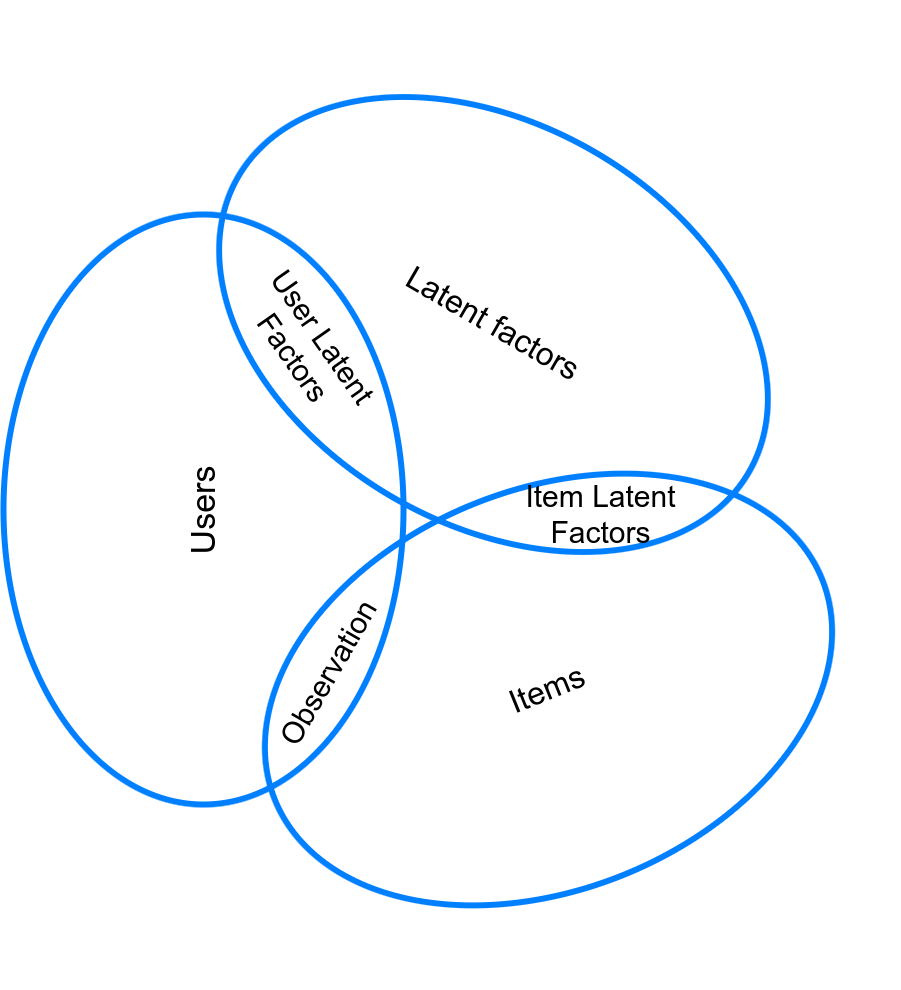
\includegraphics[width=0.5\textwidth]{images/LatentFactors.png}
	\caption{\bfseries LatentFactors}
	\label{LatentFactors}
\end{figure}

\paragraph{} In latent factors recommender systems we follow a similar approach but, in case of ALS(Alternating least squares), we are trying to find metrics that may lead us to the correct recommendation. Those metrics are not distinct, and may change in a number of iterations. Those metrics are inducted from the R matrix as we define it above. This makes this approach more tolerant to missing values, or wrong quality measures. Thus this metric as will be presented bellow is more efficient on prediction and time.
\cite{DistributedAlgorithmsAndOptimization:4}


\begin{equation}
	\min_{X,Y} \sum_{r_{ui}observed}(r_{ui}-x_{u}^{T}y_{i})^{2}
\end{equation}

\begin{equation}
	\min_{X,Y} \sum_{r_{ui}observed}(r_{ui}-x_{u}^{T}y_{i})^{2} + \lambda(\sum_{u}||x_{u}||^2 + \sum_{i}||y_{i}||^2)
\end{equation}



\paragraph{} ALS explanation.
ALS algorithm is based on the latent factors theory.As mentioned before, this means that it is not going to use the attributes given by the dataset for the movies or the users. The algorithm is going to train it self based on the rating set only.


\begin{algorithm}
	\caption{ALS for Matrix Completion}\label{ALS}
	\begin{algorithmic}[1]
		\State Initialize X,Y
		\Repeat
		\For{\texttt{u=1...n}}
		\State $x_{u} = (\sum_{r_{ui}}y_{i}y_{i}^{T} + \lambda I_k)^{-1} \sum_{r_{ui}}r_{ui}y_{i} ,\in r_{u*}$
		\EndFor
		\For{\texttt{i=1...m}}
		\State $y_{i} = (\sum_{r_{ui}}x_{u}x_{u}^{T} + \lambda I_k)^{-1} \sum_{r_{ui}}r_{ui}x_{u} ,\in r_{*i}$
		\EndFor
		\Until {convergence}
	\end{algorithmic}
\end{algorithm}